\documentclass{beamer} 
%\documentclass[handout]{beamer} 

% Michael Maier, 2014.
% CC-BY-SA 3.0 at

\usepackage[utf8]{inputenc}
\usepackage[ngerman]{babel}

\title{TransforMap - The mother of all Maps} 
\author{Michael Maier \textless Michael.Maier@mailbox.org\textgreater} 
\date{04. March 2017} 

\usetheme{Antibes}

\hypersetup{colorlinks=true,urlcolor=blue,linkcolor=white}

%\usebackgroundtemplatei{
%\includegraphics[width=\paperwidth,
%height=0.8\paperheight]{mag_map.png}
%}

\begin{document}

%\maketitle

\begin{frame} 


\begin{figure}
  \centering
  
\includegraphics[width=.5\textwidth]{logo.png}
\end{figure}

\begin{center}
\Huge{TransforMap\\}
\end{center}

\begin{center}
\Large{\emph{There are Plenty of Alternatives. \\ We make them visible.}}
\end{center}

\end{frame}


\section{Einleitung}


\begin{frame}{Vorstellung}

  \begin{itemize}
    \item Michael Maier \textless \href{mailto:Michael.Maier@mailbox.org}{Michael.Maier@mailbox.org}\textgreater
    \item Student an der TU Graz (Telematik)
\vspace{0.3cm}
    \item Linux-User (Debian/grml) seit 2004
    \item Organisiere Grazer Linuxtage seit 2011 mit
    \item OpenStreetMap als Hobby seit Juli 2010
    \item Leite den Grazer OSM-Stammtisch seit Mai 2011
\vspace{0.3cm}
    \item Freiberuflich OSM-Aufträge und Consulting
    \item Bei TransforMap seit 3 Jahren dabei
    \item Beim Elevate vor 3,5 Jahren beim Global Map Jam mit OpenStreetMap die alternative Mappingbewegung mitgestartet
  \end{itemize}
\end{frame}



% Folien zu
% * TransforMap-Geschichte, Beginn

\section{Einleitung}

\begin{frame}{TransforMap}

\begin{itemize}
  \item TransforMap ist ein internationales Projekt, gestartet März 2014 in München beim \#14MMM
\end{itemize}
 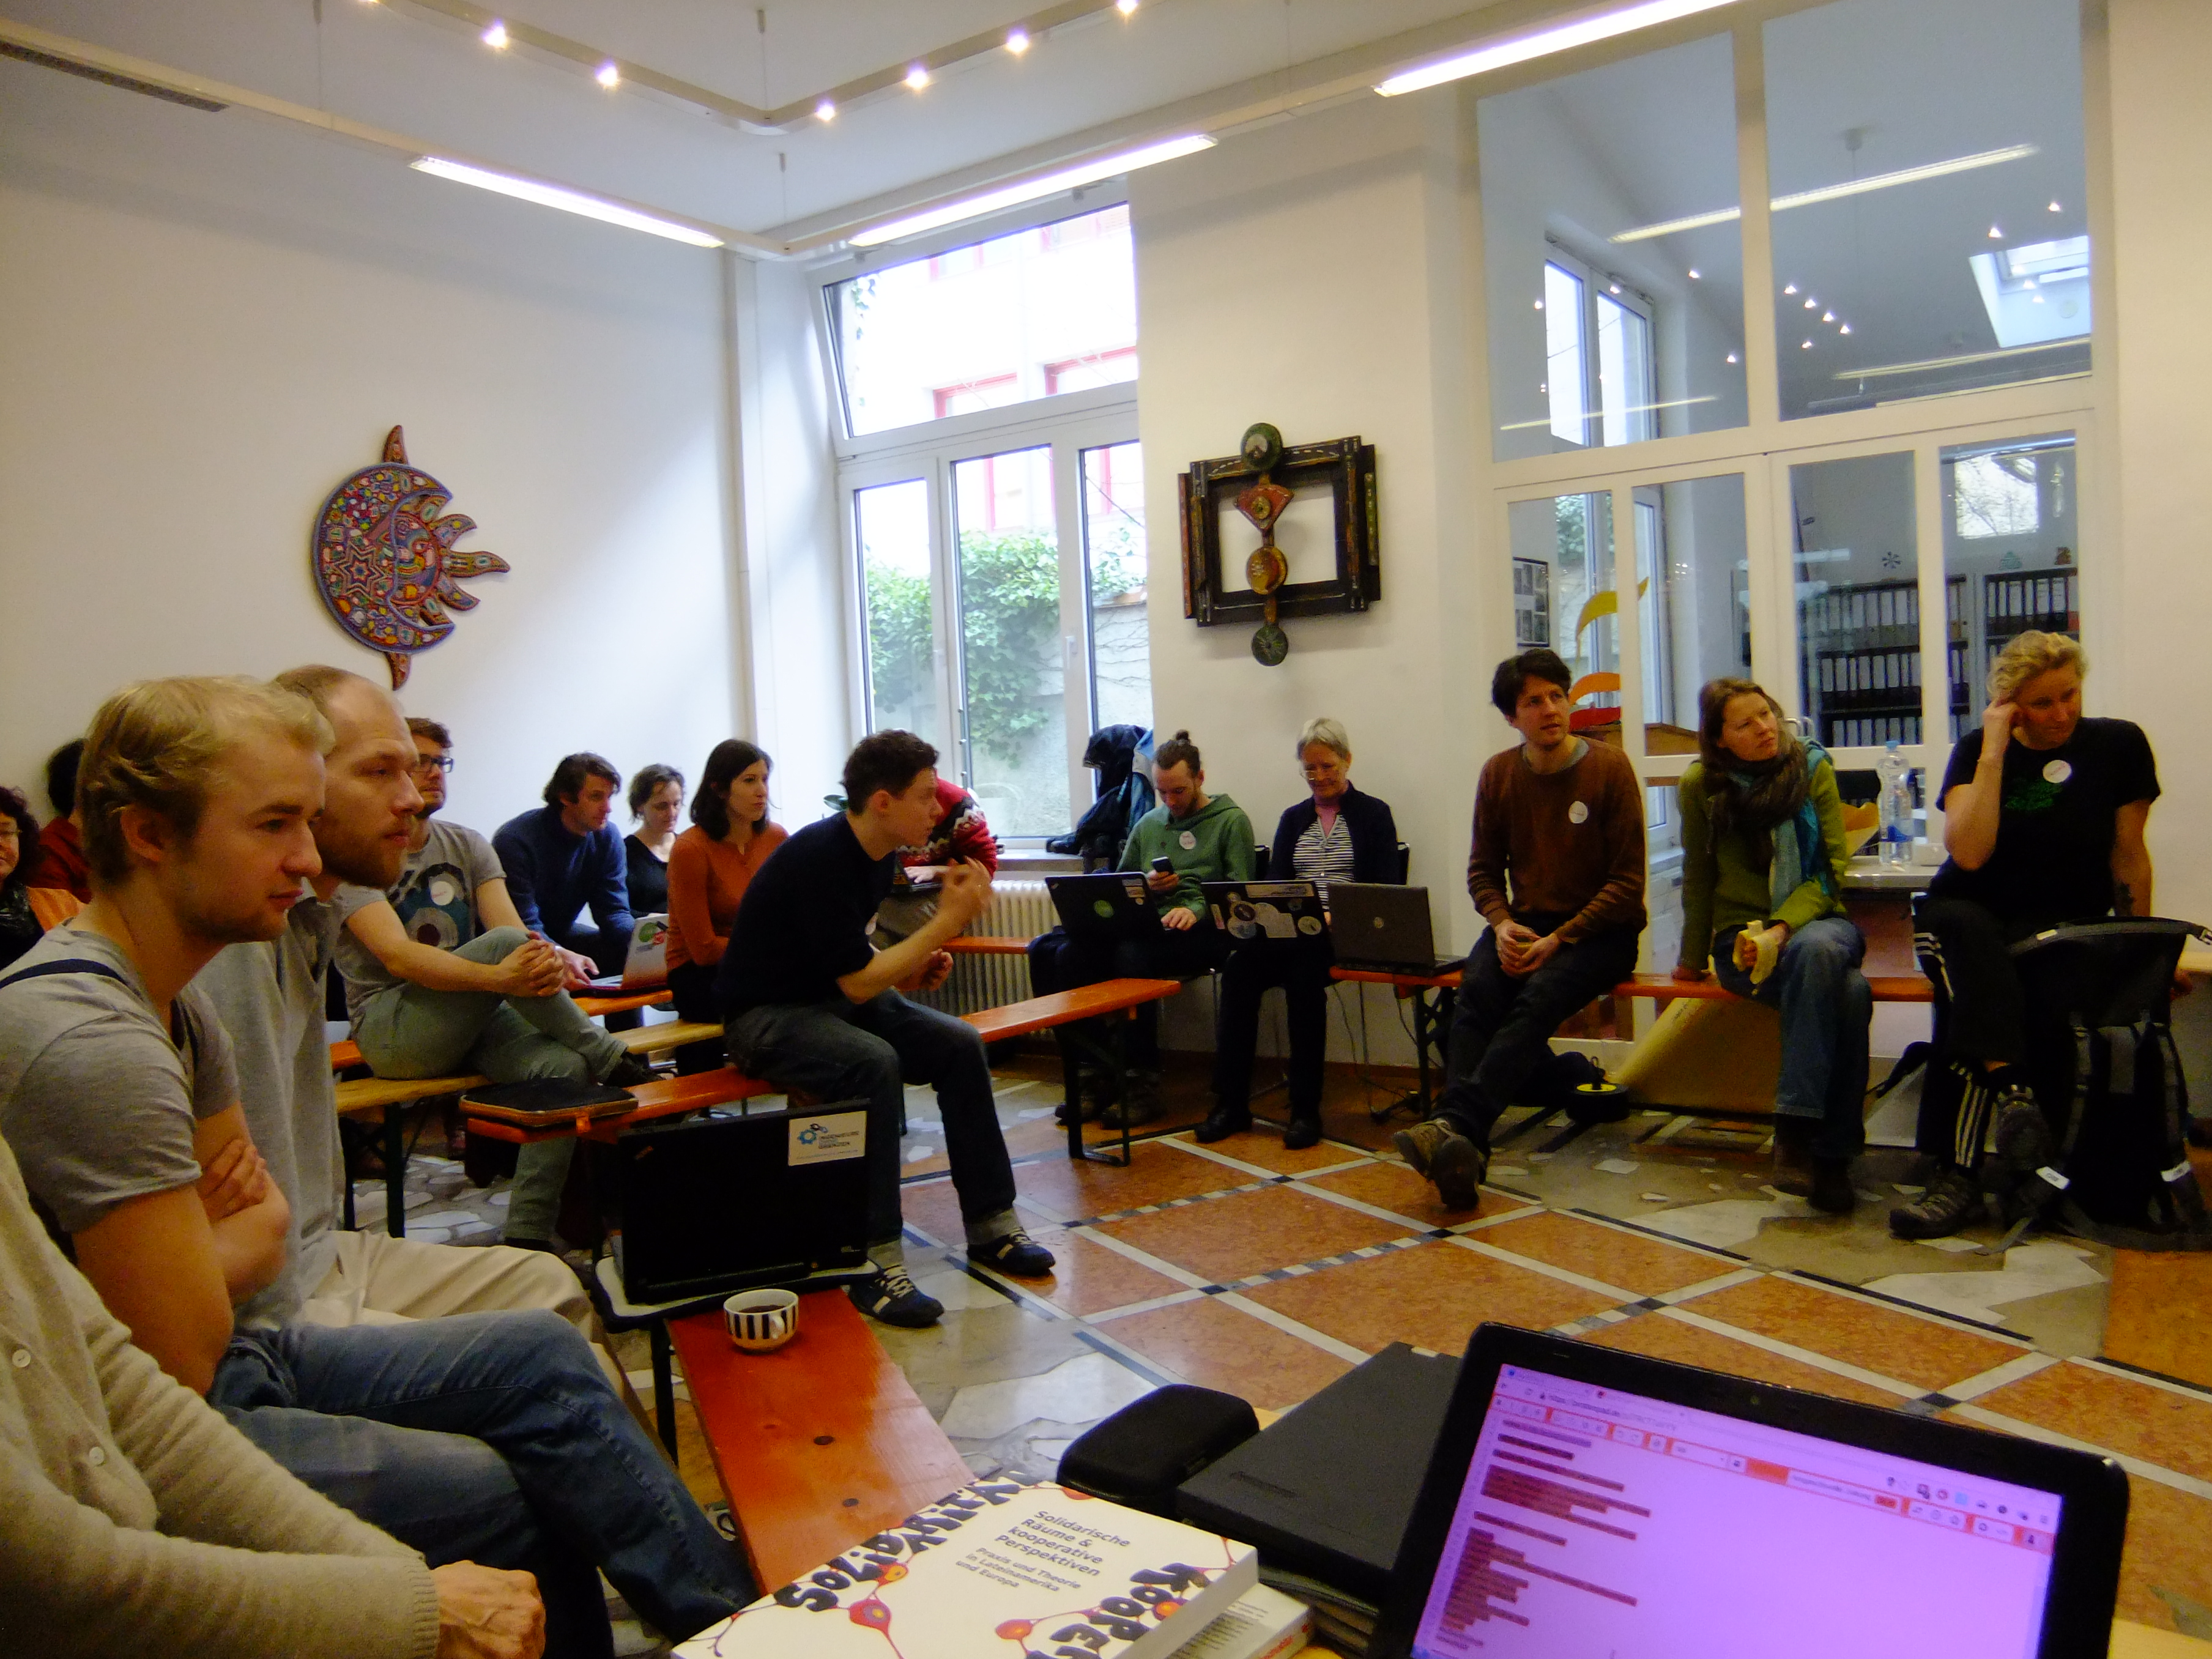
\includegraphics[width=5.5cm]{DSCF9024-gruppe.JPG}
 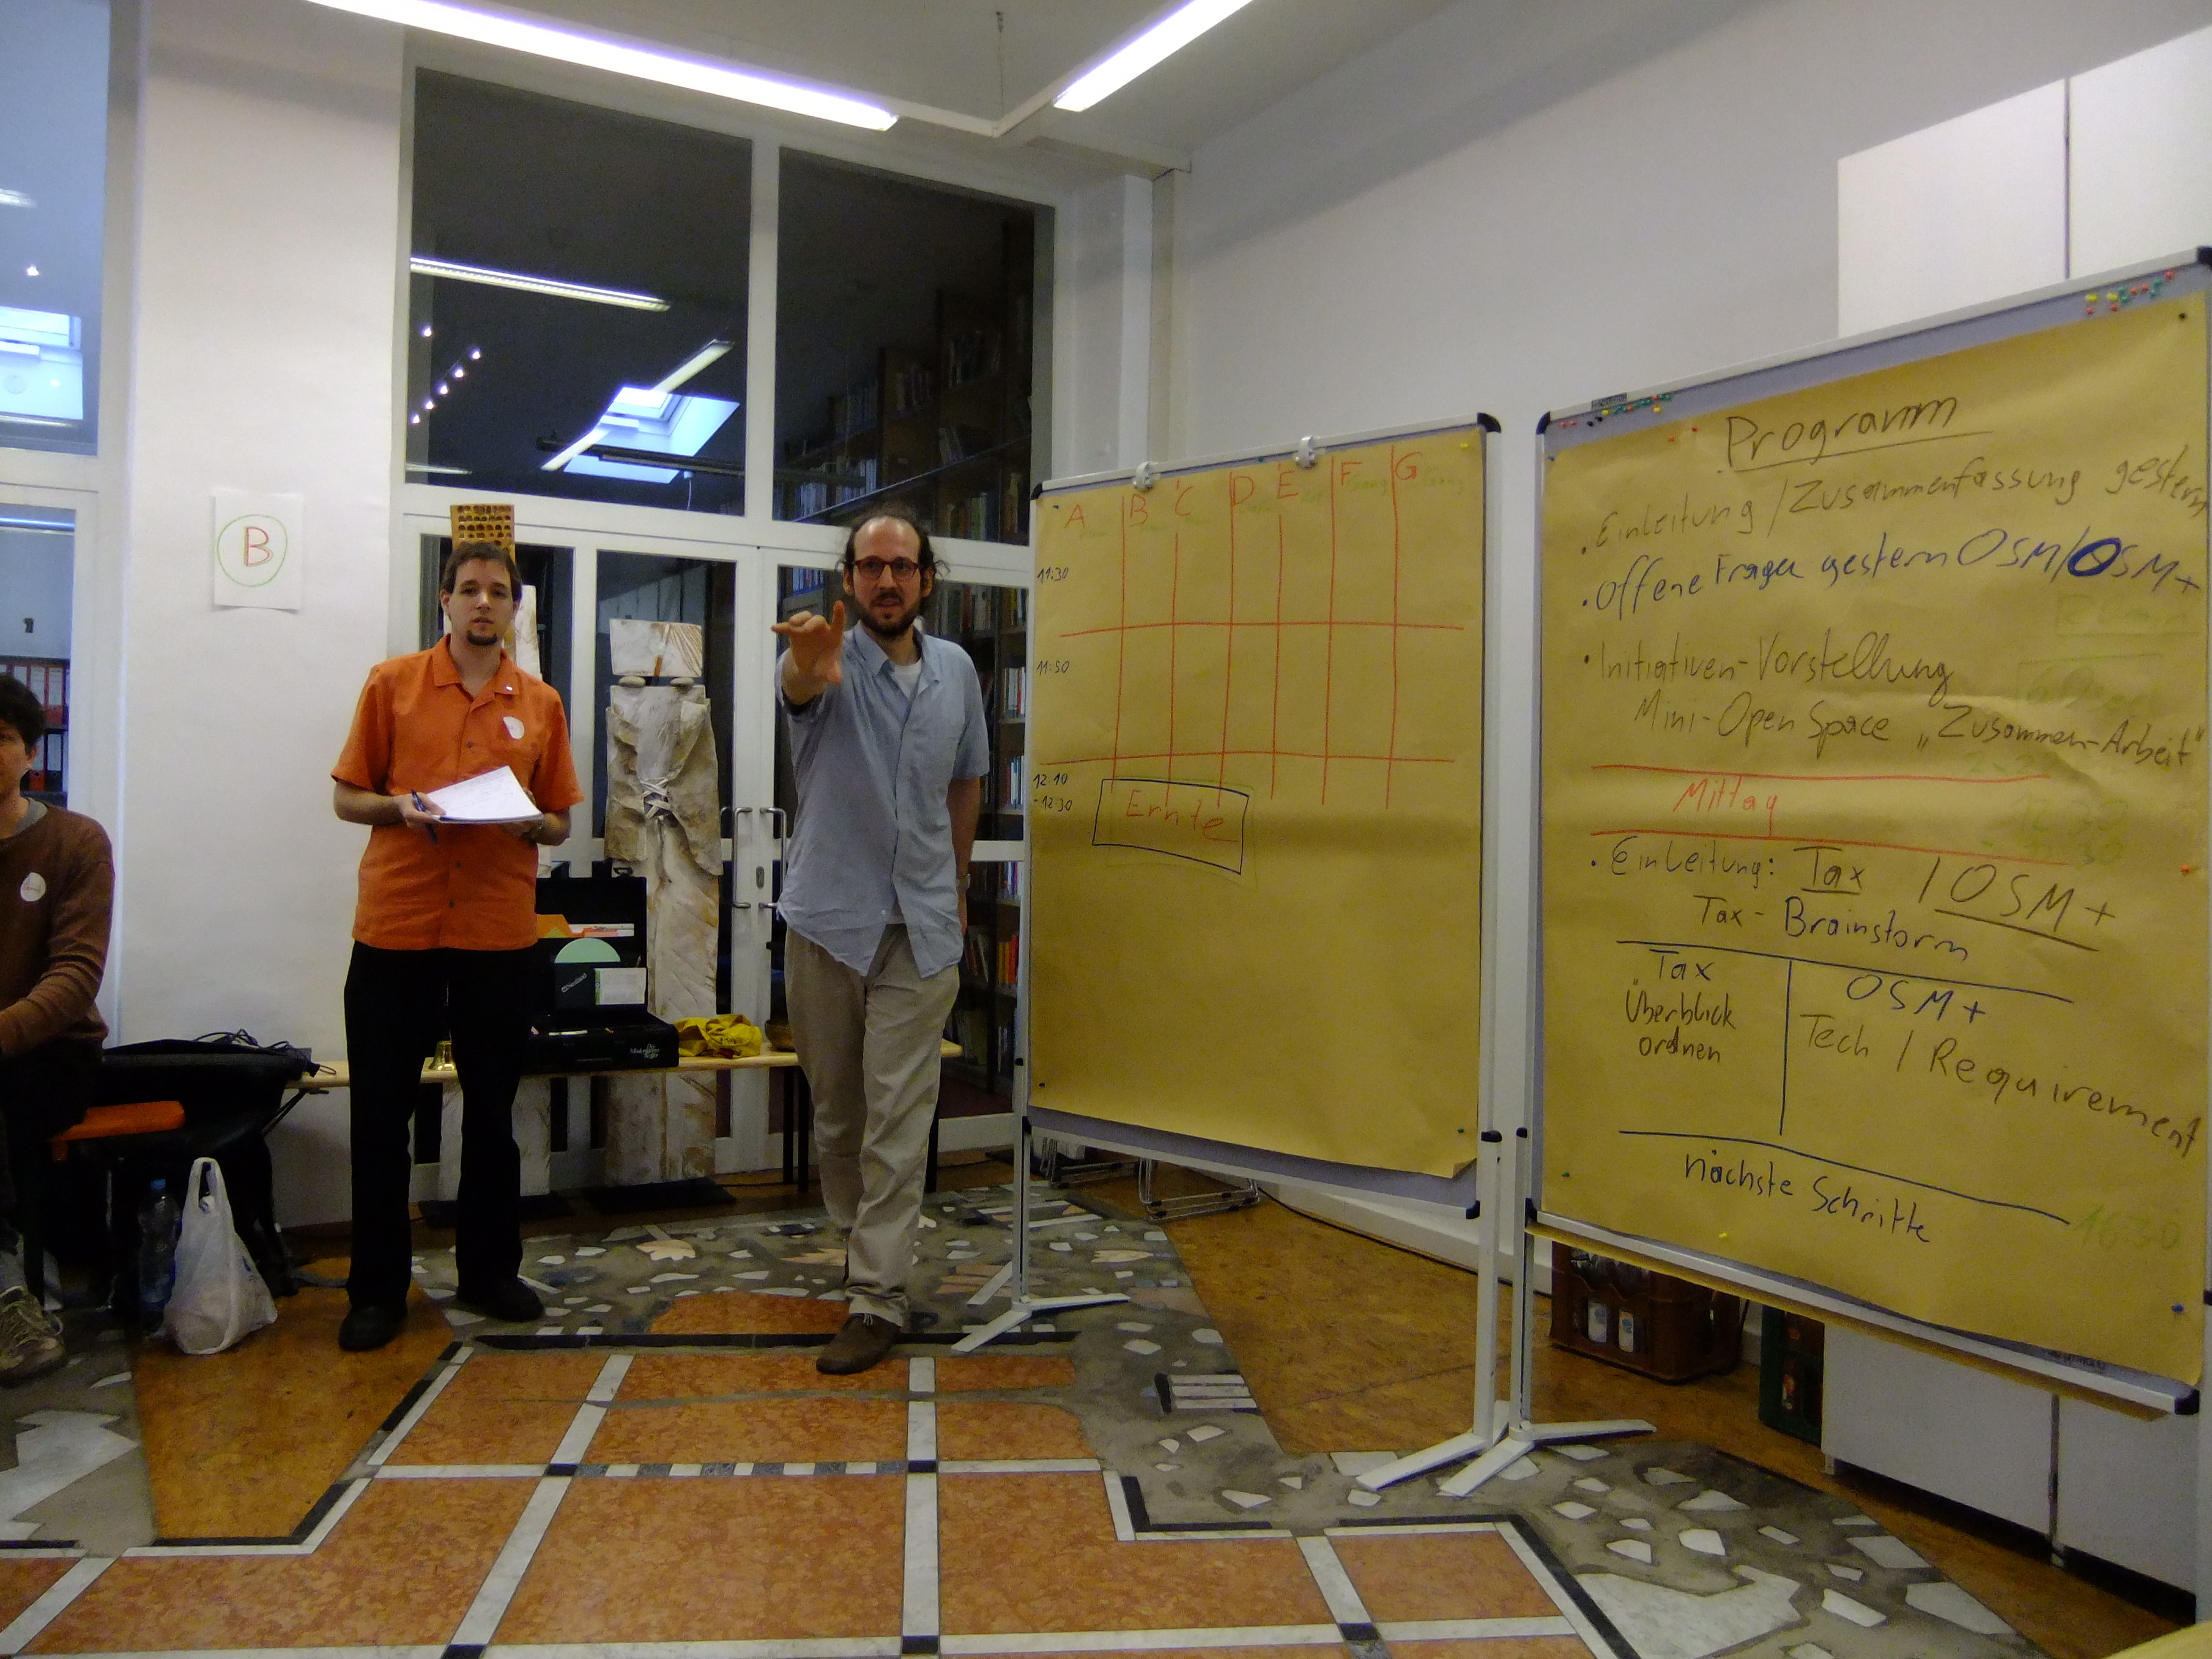
\includegraphics[width=5.5cm]{DSCF9025-josef+me.jpg}

\pause

\begin{itemize}
  \item 35 Teilnehmer, anfangs alle freiwillig
\pause
  \item später EU-Förderung (CHEST)
  \item Mapping-Teil von solidarityeconomy.eu (SSEDAS)

\end{itemize}

\end{frame}

%
% * Ziele von TransforMap
%  * Sichtbarkeit erhöhen
%  * Einheitliches Klassifizierungsschema - TM-Tax
%  * Weltweiter Standard zum mappen der alt öko

\begin{frame}{Ziele}

\begin{itemize}
  \item TAPAS: There are Plenty of Alternatives - we want to make them visible!

\pause

  \item Einheitliches Klassifizierungsschema - TransforMap Taxonomie

\pause

  \item Alternative zu Google Maps
  \item Stoppen der Fragmentierung der Karten
  \item Schaffen eines weltweiten Standards zum Mappen der alternativen Ökonomie

\end{itemize}

\end{frame}



% * TransforMap-Taxonomie

\begin{frame}{Taxonomie}

'Alternativer' Ansatz zur Klassifizierung von Initiativen - aus Sicht deren Eigenschaften:

\begin{itemize}
  \item Bedürfnisorientiert - Welche \emph{Bedürfnisse} erfüllt der Ort?

\pause

  \item Art der \emph{Interaktion} - Wie erfüllt er die Bedürfnisse?

\pause

  \item \emph{Identität} - zu welcher Strömung der Alternativen Ökonomie gehört er?

\end{itemize}

\end{frame}

% * Wie mappen?
%  * Verbindung OSM-TransforMap
%  * OSM.org: iD, JOSM
%  * TransforMap-Editor
%  * Links zwischen beiden
%   * Zuerst OSM-Objekt anlegen, speichern
%   * Dann TM-Objekt anlegen, OSM-Objekt verlinken
%   * (dann TM-Link in OSM eintragen)

\begin{frame}{Wie funktioniert TransforMap?}
  Basis ist \emph{Linked Open Data}: Links zwischen vielen Datenbanken 

 \hspace*{-1cm}  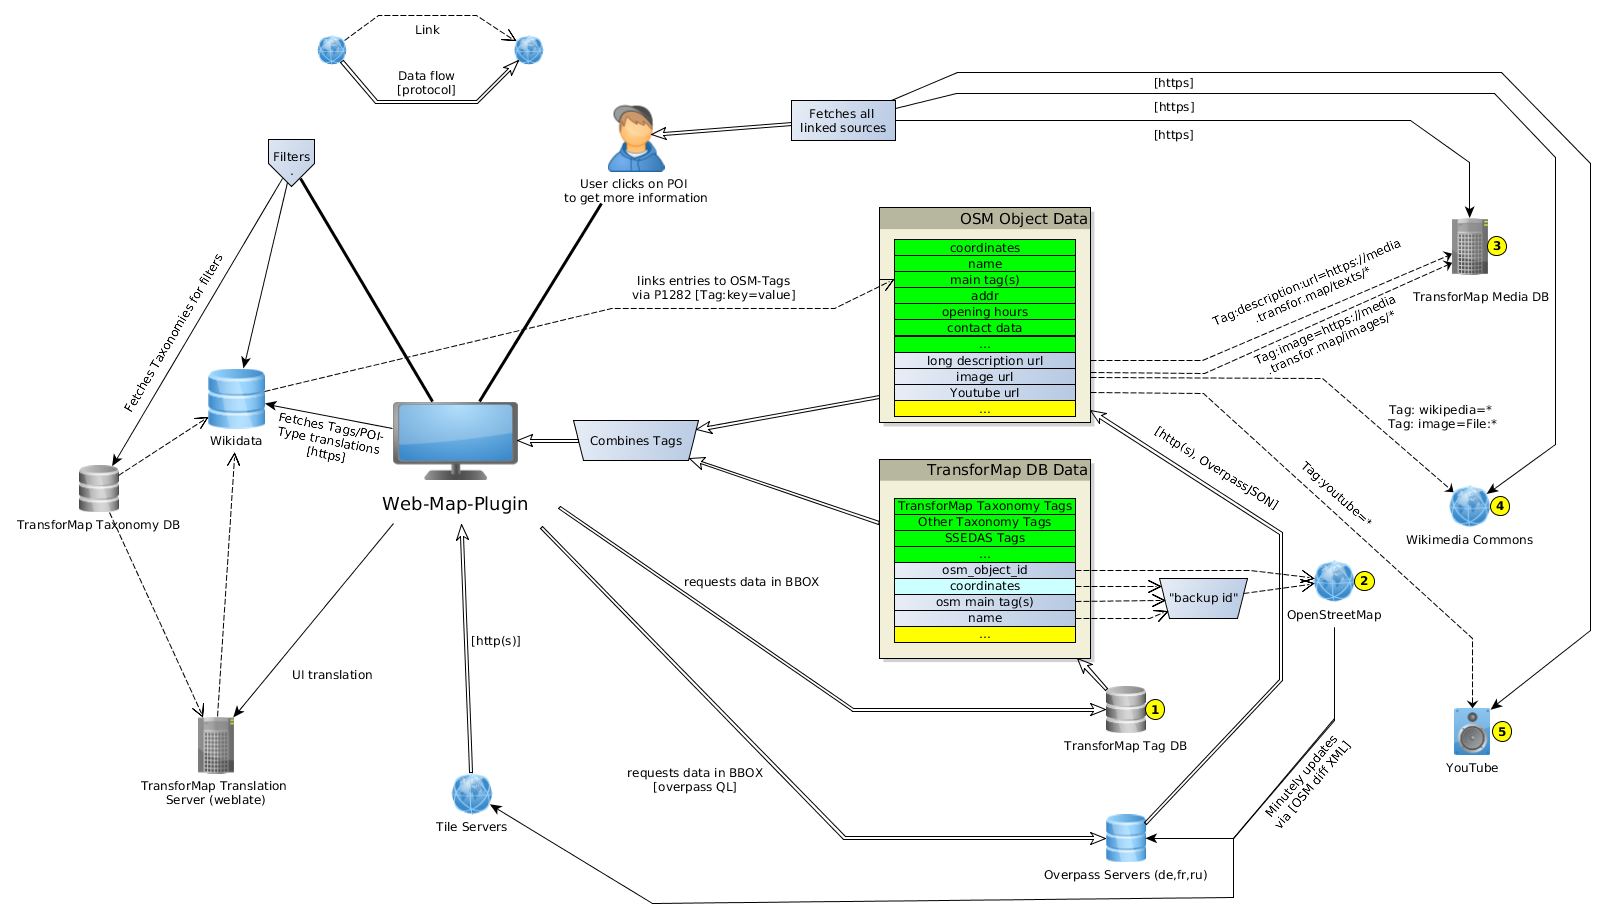
\includegraphics[width=12.5cm]{website-dataflow-overview.png}


\end{frame}

\begin{frame}{Zentrale: TransforMap Viewer}

   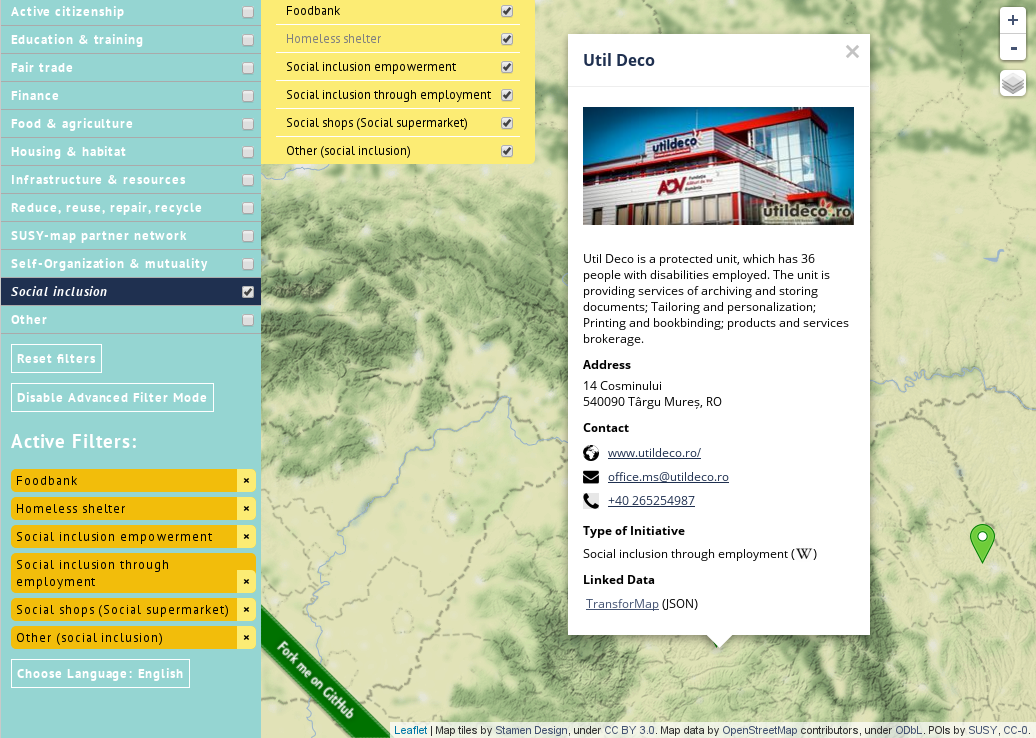
\includegraphics[width=10.5cm]{viewer.png}

\end{frame}

\begin{frame}{Datenbanken}

\begin{itemize}
  \item Geodaten, Adressen etc: OpenStreetMap
  \item TransforMap-Klassifizierung: TransforMap API
  \item Bilder: Wikimedia Commons
    \pause
  \item TransforMap-Taxonomie: Auf TransforMap Wikibase (Wikidata-Basis)
  \item Wikidata für Verbindung zu Wikipedia

\end{itemize}

\end{frame}
% * OSM: iD

\begin{frame}{OpenStreetMap Editor: iD}

 \hspace*{-1cm}  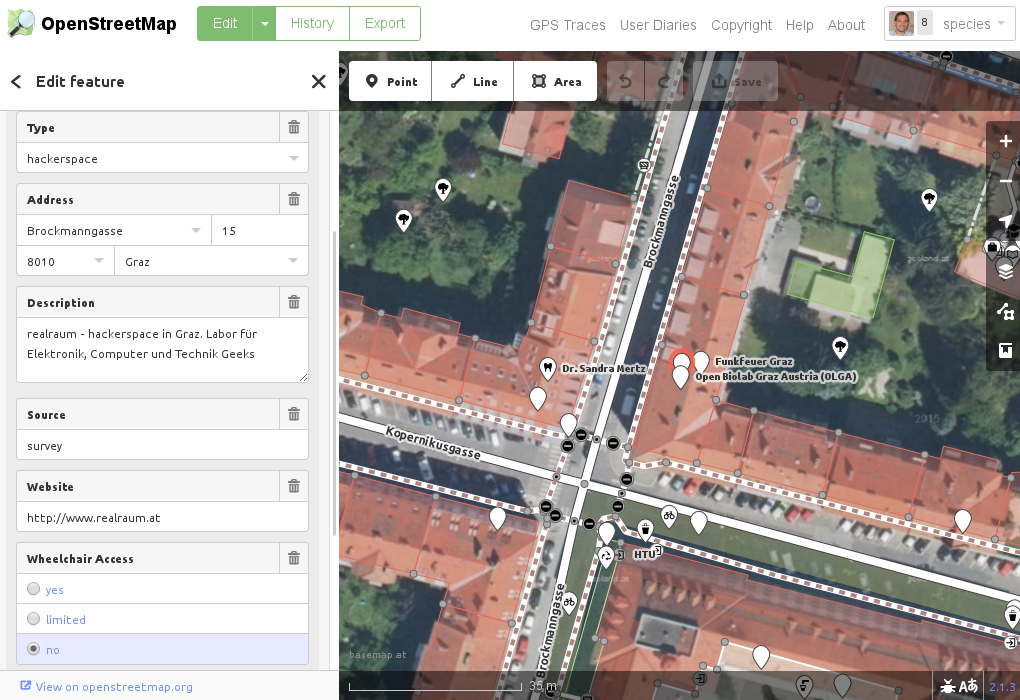
\includegraphics[width=12.5cm]{iD.png}

\end{frame}
%
% * TransforMap-Editor


\begin{frame}{TransforMap Editor}

 \hspace*{-1cm}  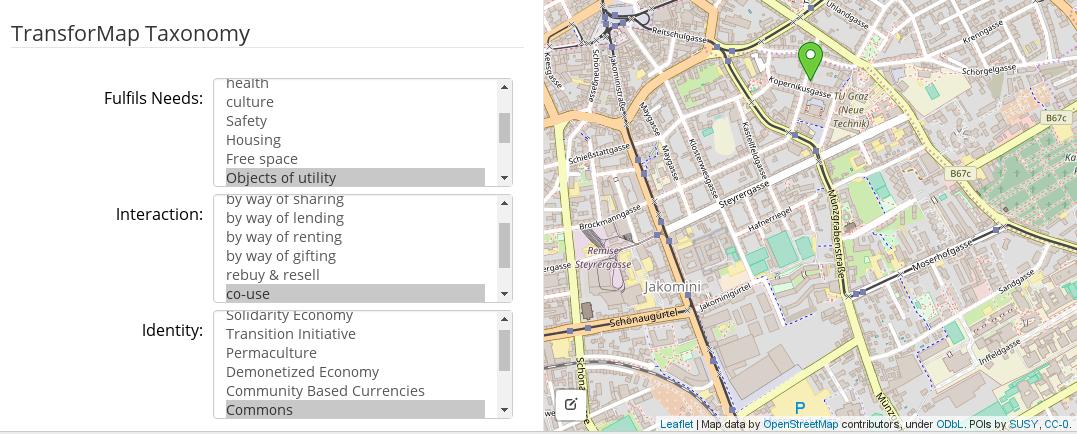
\includegraphics[width=12.5cm]{tm.png} \\
 \hspace*{-1cm}  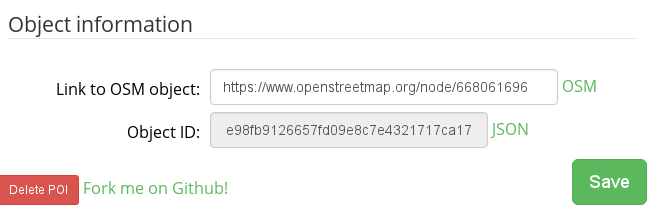
\includegraphics[width=6.5cm]{tm2.png}

\end{frame}


\section{Ende}

\begin{frame}{Vielen Dank für die Aufmerksamkeit!}

  Folien zu Map the Change am Elevate März 2017
\vspace{0.8cm}

Erstellt mittels \LaTeX Beamer, Quelltext: \href{https://github.com/species/vortrag-transformap-elevateM17}{Github/species/vortrag-transformap-elevateM17}.
\vspace{0.8cm}

\href{mailto:michael.maier@mailbox.org}{Michael Maier}

Twitter: \href{https://twitter.com/osmgraz}{@osmgraz}
\vspace{0.8cm}

Folien unter: 
\includegraphics[width=1cm]{cc-by-sa.pdf}. 

Alle Karten ODbL, OpenStreetMap Contributors.

Alle Daten Public Domain, TransforMap Contributors.

\vspace{0.8cm}


\end{frame}



\end{document}
